\documentclass{article}

%\usepackage[final]{nips_2016_modified}  % Use this for final version
\usepackage{nips_2016_modified}  % Use this for draft

\usepackage[utf8]{inputenc} % allow utf-8 input
\usepackage[T1]{fontenc}    % use 8-bit T1 fonts
\usepackage{hyperref}       % hyperlinks
\usepackage{url}            % simple URL typesetting
\usepackage{booktabs}       % professional-quality tables
\usepackage{amsmath}
\usepackage{amsfonts}       % blackboard math symbols
\usepackage{mathtools}
\usepackage{nicefrac}       % compact symbols for 1/2, etc.
\usepackage{microtype}      % microtypography
%\usepackage{algorithm}
%\usepackage{algpseudocode}
\usepackage{graphicx}
\usepackage{float}\usepackage{caption}
\usepackage{outlines}
\usepackage{tikz}
\usepackage{dsfont}
\usepackage{empheq}
%\usepackage{geometry}
%\geometry{margin=1.5in}

\usetikzlibrary{bayesnet,positioning}

\newcommand{\nth}{^{\text{th}}}
\newcommand{\len}{\mathrm{len}}
\newcommand{\indicator}{\mathds{1}}

%\allowdisplaybreaks

\title{Hierarchical Topic Models}

\author{
  Andrew Leverentz \\
  \texttt{aleveren@eng.ucsd.edu} \\
}

\begin{document}

\maketitle

\begin{abstract}
In this paper, we survey techniques for automatically inferring hierarchical structures from unlabeled collections of text documents.
We begin with an overview of probabilistic topic modeling, as implemented in models such as Probabilistic Latent Semantic Analysis (PLSA) and Latent Dirichlet Allocation (LDA).
After examining some limitations of these models, we discuss a line of research which has extended the LDA model and has attempted to address some of its weaknesses.
This approach treats topics as belonging to a potentially infinite tree; in this context, Bayesian non-parametric techniques based on Dirichlet Processes are used to automatically select the structure of the tree.
We compare and contrast two topic models that have been used for this approach---the Nested Chinese Restaurant Process (NCRP) and the Nested Hierarchical Dirichlet Process (NHDP)---and we discuss several inference algorithms that have been published in the literature.
\end{abstract}

%%%%%%%%%%%%%%%%%%%%%%%%%%%%%%%%
\section{Introduction}

In recent decades, large-scale digital archives and information-sharing networks such as the World Wide Web have led to the creation of vast collections of electronic textual data.
As these collections grow, the problem of efficiently discovering relationships between documents, or between  user queries and documents, has become more prominent.
The field of \emph{topic modeling} has produced several automated approaches to solving this problem.

One underlying theme of topic modeling is the notion that words with similar meanings tend to co-occur with similar sets of words.
However, due to ambiguities in natural language and variations between different authors, these co-occurrence patterns are not rigid and deterministic.
To address this, many techniques within the field of topic modeling use a probabilistic framework.
In this probabilistic framework, topics are represented as discrete probability distributions over vocabulary words, and documents may contain mixtures of multiple topics.

In subsequent sections, we briefly review the origins of Latent Dirichlet Allocation (LDA) and the probabilistic framework for topic modeling.
Then, we trace the development of a line of research which extends the LDA model and is capable of producing not just a flat collection of topics but a nested hierarchy of topics.
We conclude with a discussion of potential avenues for future research.

%%%%%%%%%%%%%%%%%%%%%%%%%%%%%%%%
\section{Motivation}
Two of the main applications of topic models are (1) discovering relations between documents and (2) indexing large collections of documents.

\paragraph{Discovering relations between documents:}
We often want to determine which sets of documents within a corpus share the same topic or subject matter.
One approach is to formulate this as a clustering task with soft cluster assignments---also known as a \emph{mixed membership model}---where each document can be assigned to a mixture of multiple topics or clusters.
For example, a news article about a national politician's economic policies might be represented as a mixture between topics corresponding to both \emph{politics} and \emph{economics}.
Thus, if we are looking for related documents, we could return the set of documents which also contain some significant proportion of either \emph{politics} or \emph{economics}.

\paragraph{Indexing large collections of documents:}
In the context of information retrieval, the task is to take a user query (expressed perhaps as a collection of keywords or as a natural-language sentence) and efficiently find a set of documents which are deemed most relevant to that query.

Both of these tasks are complicated by ambiguities in natural language.
In particular, \emph{synonymy} (in which multiple words have nearly identical meanings) and \emph{polysemy} (in which a single word may have multiple meanings, depending on the context) make it difficult to draw conclusions about relationships between documents based on the specific set of words used in each document.
For example, two closely related documents might express nearly the same concept using completely different words, whereas two unrelated documents might coincidentally both use a particular word in different senses.
Because of this, it is necessary to move beyond superficial representations of documents (such as strings of characters or tokens, or histograms of vocabulary words) and instead represent documents using some notion of \emph{latent semantics}, or underlying meaning.

Topic models accomplish this by treating topics as probability distributions over the vocabulary and allowing documents to draw from mixtures of multiple topics.
For example, a topic relating to sports would assign relatively high probability to words such as ``player,'' ``team,'' and ``game.''
Similarly, a topic about medicine would assign relatively high probability to ``doctor,'' ``illness,'' and ``pharmacy.''
Then, a document about a basketball player recovering from an injury might consist of $70\%$ \emph{sports} and $30\%$ \emph{medicine}, whereas a document about physical therapy for athletes might consist of $70\%$ \emph{medicine} and $30\%$ \emph{sports}.

Hierarchical topic models extend this idea by acknowledging that whether or not two documents share the same topic may depend on the level of abstraction that the user is interested in.
By explicitly treating the set of available topics as a tree, hierarchical topic models can therefore represent documents as mixtures of nested topics at varying levels of abstraction.
For example, in some contexts, we might consider articles about the San Diego Padres and articles about the Chicago Bulls to belong to the same topic (namely, \emph{sports}), whereas in other contexts, they belong to distinct topics (\emph{baseball} versus \emph{basketball}).
Thus, \emph{baseball} and \emph{basketball} could be considered subtopics under the broader topic of \emph{sports}.
For indexing tasks, hierarchical topic models allow the possibility of expanding or narrowing the set of relevant documents, depending on the level of abstraction desired by the user.
For example, when searching for documents related to the keywords ``Alan Turing,'' the default system behavior might be to display documents related to \emph{computer science}, with the option of narrowing matches to a more specific subtopic (e.g., \emph{British computer scientists}) or expanding matches to a more general supertopic (e.g., \emph{science and engineering}).

%%%%%%%%%%%%%%%%%%%%%%%%%%%%%%%%
\section{Probabilistic Topic Models}

Before we discuss models which can generate hierarchies of topics, we will first discuss two probabilistic models which generate ``flat'' (that is, non-nested) collections of topics.
These models are Probabilistic Latent Semantic Analysis (PLSA) and Latent Dirichlet Allocation (LDA).

\subsection{A Non-Probabilistic Precursor: Latent Semantic Analysis}

The first of these, PLSA, was inspired by an earlier, non-probabilistic model known as Latent Semantic Analysis (LSA), which was introduced in \cite{deerwester1990lsa}.
In LSA, a corpus of documents is summarized as a matrix; each column of this matrix represents a document, each row represents a term in the vocabulary, and each entry represents number of times a given term appears in a given document.
In mathematical notation, we have a matrix $M$ such that the entry $M_{i,j}$ represents the number of times that the $i\nth$ vocabulary word appears in the $j\nth$ document.
If the corpus contains a sufficiently diverse set of documents, then most documents will only contain a small subset of the full vocabulary, and the resulting matrix will be sparse.
After constructing this matrix, we may optionally transform it according to per-term and per-document statistics.
That is, if $M$ is an $N \times D$ matrix, we compute a new $N \times D$ matrix $X$ whose entries are given by
\begin{align}
X_{i,j} &= f(M_{i,j}, M_{1:D,j}, M_{i,1:N}).
\end{align}
Several variants of LSA exist which use different transformations in this step, as described in \cite{wiki:lsa}, although the original paper \cite{deerwester1990lsa} uses an untransformed matrix, with $X = M$.
Then, the singular value decomposition (SVD) of the matrix $X$ is computed.
This represents the matrix as a product of three matrices:
\begin{align}
X &= U \Sigma V^\top
\end{align}
Here, $U$ and $V$ are matrices of orthogonal column vectors.
In $U$, each row corresponds to a term in the vocabulary, and in the transposed matrix $V^\top$, each column corresponds to a document.
Moreover, $\Sigma$ is a diagonal matrix containing scaling factors known as \emph{singular values}.
If we compute the SVD using a low-rank approximation, this corresponds to truncating the number of columns in $U$ and the number of rows in $V^\top$.
At the same time, we also discard all but the largest singular values in $\Sigma$.
The truncated rows from $U$ (corresponding to terms) and truncated columns from $V^\top$ (corresponding to documents) are known as \emph{latent semantic vectors}.
We can view these vectors as concise representations of terms and documents in a low-dimensional \emph{latent semantic space}.
Using these representations, we can measure the similarity between pairs of documents by computing a normalized dot product (also known as \emph{cosine similarity}) of the corresponding latent semantic vectors.

However, one major limitation of this model is that the latent semantic vectors corresponding to terms and documents do not have an intuitive interpretation.
Consequently, there are relatively few theoretical principles to guide the design of algorithms for (non-probabilistic) LSA.
For example, selecting the transformation $f$ which maps $M$ to $X$ must typically be done by trying many variations and then determining which one happens to yield the most reasonable-looking results in practice.
We will see that subsequent models have addressed this limitation by using a probabilistic framework.

Lastly, we note that this model, as with many other topic models, uses the \emph{bag-of-words} simplification, in which the specific sequence of words in a document is ignored, and all that matters is the frequency of terms within each document.
Topic models which eliminate the bag-of-words simplification are beyond the scope of this survey, but they constitute an active area of research.

\subsection{Probabilistic Latent Semantic Analysis}

In abstract terms, Probabilistic Latent Sematic Analysis (PLSA) takes a conceptual approach that is similar to LSA, but in this case the latent semantic representations of topics associated with terms and documents are combined using a probabilistic model, rather than simply a linear algebraic one.
PLSA, introduced in Hofmann \cite{hofmann1999plsa}, uses an \emph{aspect model} to represent documents as probabilistic mixtures of topics.
It is worth noting that the ``A'' in LSA and PLSA is sometimes replaced with ``I'' for ``Indexing'' when the primary goal is to efficiently retrieve documents related to a given user query.
Thus the terms ``LSI'' and ``PLSI'' are often used in the information retrieval research community.

In this model, the observed dataset is a collection of $D$ documents, and for each $d \in \{1, \ldots, D\}$, document $d$ contains $N_d$ words.
We assume that these documents share a fixed vocabulary $\mathcal V$, which is a set of words.
Furthermore, we assume that there are a total of $K$ available topics, each of which is represented as a distribution over the words in the vocabulary.
More concretely, we represent each topic $k \in \{1, \ldots, K\}$ as a vector $\theta_k$ of length $|\mathcal V|$ whose components sum to 1.
Each document $d$ is associated with a mixture of topics $\phi_d$, which we represent as a vector of length $K$ whose components sum to 1, and which we view as a probability distribution over topics.
As with LSA, we will use the bag-of-words assumption to ignore the order in which words appear.

Once we have defined topic vectors $\theta_k$ for $k \in \{1, \ldots, K\}$ and per-document topic mixtures $\phi_d$ for $d \in \{1, \ldots, D\}$, we assume that documents are generated according to the following probabilistic procedure:
\begin{outline}
\1 For each document $d \in \{1, \ldots, D\}$:
  \2 For each word-slot $n \in \{1, \ldots, N_d\}$:
    \3 Select a topic $z_{d,n} \in \{1, \ldots, K\}$ according to the current document's topic mixture $\phi_d$.
    \3 Select a word $t_{d,n} \in \{1, \ldots, |\mathcal V|\}$ from the vocabulary according to the topic vector indexed by $z_{d,n}$.
\end{outline}

This model can be summarized by the following probability distributions:
\begin{align}
z_{d,n} &\sim \text{Categorical}(\phi_d) &\qquad&\text{for the $n\nth$ word in document $d$} \\
t_{d,n} &\sim \text{Categorical}(\theta_{z_{d,n}}) &\qquad&\text{for the $n\nth$ word in document $d$}
\end{align}
Figure~\ref{fig:plate-plsa} illustrates this model using plate-diagram notation.
In this notation, unshaded circles represent latent (i.e., unobserved) random variables, and shaded circles represent observed random variables.
Uncircled variables denote hyperparameters, which are variables with no associated probability distribution.
Edges represent conditional dependencies between variables, which correspond to the probability distributions listed above.
Finally, the rectangular plates denote repetitions of the nodes and edges that they contain.

%%%%
\begin{figure}[htb]
%
\centering
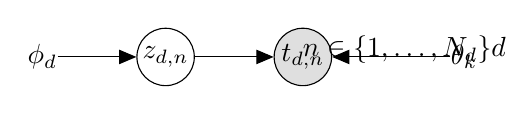
\begin{tikzpicture}
\node[obs] (t) {$t_{d,n}$};
\node[const, right=1.5cm of t] (theta) {$\theta_k$};
\node[latent, left=of t] (z) {$z_{d,n}$};
\node[const, left=of z] (phi) {$\phi_d$};

\edge{phi}{z};
\edge{theta}{t};
\edge{z}{t};

\centeredPlate{word-plate}{(t)(z)}{$n \in \{1, \ldots, N_d\}$};
\centeredPlate{doc-plate}{(word-plate)(phi)}{$d \in \{1, \ldots, D\}$};
\centeredPlate{topic-plate}{(theta)}{$k \in \{1, \ldots, K\}$};
\end{tikzpicture}
%
\caption{Plate diagram for the PLSA model.}
\label{fig:plate-plsa}
\end{figure}
%%%%

Thus, the joint probability of the PLSA model is
\begin{align}
p(\vec{t}, \vec{z})
&= \prod_{d=1}^D \prod_{n=1}^{N_d} p(t_{d,n} \mid z_{d,n}) \, p(z_{d,n}) \\
&= \prod_{d=1}^D \prod_{n=1}^{N_d} \theta_{z_{d,n}, t_{d,n}} \, \phi_{d, z_{d,n}}
\end{align}
Within this framework, it becomes possible to infer the latent topic mixture of each document using a maximum-likelihood optimization algorithm.
One such option is the expectation--maximization (EM) algorithm, which was introduced in Dempster et al \cite{dempster1977em}.
We omit the details of this algorithm, since it is not applicable to the more complex hierarchical topic models discussed below.
However, as outlined in Barber \cite{barber2012bayesian}, the EM algorithm generally consists of alternating between estimating distributions over the latent topic assignments $z_{d,n}$ (known as the ``E step'') and maximizing a quantity related to the likelihood of the data (known as the ``M step'').

%The following outline of the EM algorithm follows the exposition given in Barber \cite{barber2012bayesian}.

% In general, maximum-likelihood optimization involves finding the value of unobserved model parameters which maximizes the probability (or, equivalently, the log-probability) of the observed data.
% For the PLSA model, the EM algorithm involves optimizing quantities of the following form:
% \begin{align}
% \arg\max_{\theta, \phi} \sum_{d=1}^D \sum_{n=1}^{N_d} E_{z_{d,n} \sim q(\cdot \mid t_{d,n})} \left[ \log p(t_{d,n}, z_{d,n}) \right]
% \label{eq:plsa-optimize}
% \end{align}
% Here, the expectation is taken with respect to the latent variables $z_{d,n}$, but not the observed variables $t_{d,n}$.
% Moreover, rather than computing the expectation using the true posterior distribution ${p(z_{d,n} \mid t_{d,n})}$, the expectation is computed using an estimate ${q(z_{d,n} \mid t_{d,n})}$, which we update repeatedly throughout the algorithm based on our current estimate for the parameters $\theta$ and $\phi$.
% In particular, we keep track of the current estimated parameter values ($\theta$ and $\phi$) and alternate between an ``E~step,'' which updates estimates for ${q(z_{d,n} \mid t_{d,n})}$, and an ``M~step,'' which updates the estimates for $\theta$ and $\phi$ by performing the optimization in equation~\eqref{eq:plsa-optimize}.
% For PLSA, this happens to be a constrained optimization, since the values of $\phi_d$ for each document $d$ and $\theta_k$ for each topic $k$ must be probability distributions, with non-negative components that sum to 1.
% We can compute the E~step using Bayes' rule:
% \begin{align}
% q(z_{d,n} \mid t_{d,n})
% &= \frac{\theta_{z_{d,n}, t_{d,n}} \, \phi_{d, z_{d,n}}}
%         {\sum_{k=1}^K \theta_{k, t_{d,n}} \, \phi_{d, k}}
% \end{align}
% The M~step is possible to compute using gradients and Lagrange multipliers:
% \begin{align}
% \theta_{i,j} &\propto \sum_{d=1}^D \sum_{n=1}^{N_d} q(z_{d,n} = i \mid t_{d,n} = j) \indicator [t_{d,n} = j] \\
% \phi_{d,k} &\propto \sum_{n=1}^{N_d} q(z_{d,n} = k \mid t_{d,n})
% \end{align}
% Combining these results yields an iterative procedure for obtaining maximum-likelihood estimates for $\theta$ and $\phi$:
% initialize $\theta$ and $\phi$ to a reasonable guess, then repeat the E and M steps until the estimates converge.

\subsection{Latent Dirichlet Allocation}

Since the PLSA model does not specify probability distributions for the unobserved parameters $\phi_d$ and $\theta_k$, Bayesian inference methods are not applicable.
It is also prone to overfitting, meaning that its results can be overly sensitive to the randomness that is involved in generating or sampling the training data.
To address these problems, Latent Dirichlet Allocation (LDA) extends PLSA by using the Dirichlet distribution as a Bayesian prior on the space of discrete probability distributions.
A simpler version of this model was introduced in Blei et al \cite{blei2003lda}, although the term ``LDA'' now typically refers to the variant proposed by Griffiths and Steyvers \cite{griffiths2004lda}.

Recall that an $m$-dimensional Dirichlet distribution is a continuous distribution over the set of length-$m$ vectors whose components are non-negative and sum to one.
In other words, it is a meta-distribution over discrete distributions over a set of $m$ points.
The Dirichlet distribution is parameterized by a length-$m$ vector of positive real numbers, $\vec \alpha = (\alpha_1, \ldots, \alpha_m)$, and its density over the $m$-dimensional simplex is proportional to
\begin{align}
\text{Dirichlet}(\vec x \mid \vec \alpha) &\propto \prod_{i=1}^m x_i^{(\alpha_i-1)}
\end{align}
The Dirichlet distribution is a higher-dimensional generalization of the beta distribution:
\begin{align}
\text{Beta}(x \mid \alpha_1, \alpha_0) &\propto x^{(\alpha_1-1)} (1-x)^{(\alpha_0-1)}
\end{align}

The generative model used in LDA is given by:
\begin{alignat}{2}
\theta_k &\sim \text{Dirichlet}(\alpha) &\qquad&\text{for each topic $k$} \\
\phi_d &\sim \text{Dirichlet}(\beta) &\qquad&\text{for each document $d$} \\
z_{d,n} &\sim \text{Categorical}(\phi_d) &\qquad&\text{for the $n\nth$ word in document $d$} \\
t_{d,n} &\sim \text{Categorical}(\theta_{z_{d,n}}) &\qquad&\text{for the $n\nth$ word in document $d$}
\end{alignat}
In other words, the per-topic probability distributions over the vocabulary ($\theta_k$) are i.i.d.\ draws from a Dirichlet distribution.
Then, each document is associated with a random draw $\phi_d$ from another Dirichlet distribution; this represents the proportion of topics present in document $d$.
Within each document, we select a topic indicator $z_{d,n}$ for each word according to the probabilities in the vector $\phi_d$, and the vocabulary word $t_{d,n} \in \mathcal V$ at the $n\nth$ position is selected according to the probabilities in the vector $\theta_{z_{d,n}}$.
The plate diagram for this model is shown in Figure~\ref{fig:plate-lda}.

%%%%
\begin{figure}[htb]
%
\centering
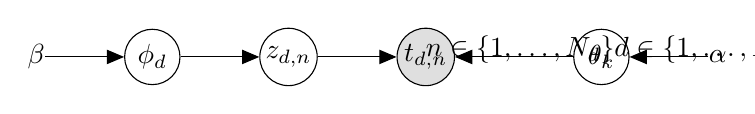
\begin{tikzpicture}
\node[obs] (t) {$t_{d,n}$};
\node[latent, right=1.5cm of t] (theta) {$\theta_k$};
\node[latent, left=of t] (z) {$z_{d,n}$};
\node[latent, left=of z] (phi) {$\phi_d$};
\node[const, right=of theta] (alpha) {$\alpha$};
\node[const, left=of phi] (beta) {$\beta$};

\edge{alpha}{theta};
\edge{phi}{z};
\edge{beta}{phi};
\edge{theta}{t};
\edge{z}{t};

\centeredPlate{word-plate}{(t)(z)}{$n \in \{1, \ldots, N_d\}$};
\centeredPlate{doc-plate}{(word-plate)(phi)}{$d \in \{1, \ldots, D\}$};
\centeredPlate{topic-plate}{(theta)}{$k \in \{1, \ldots, K\}$};
\end{tikzpicture}
%
\caption{Plate diagram for the LDA model}
\label{fig:plate-lda}
\end{figure}
%%%%

The LDA model has two main advantages over the PLSA.
First, it creates a fully generative model which specifies how documents can be generated.
Hence, it is possible to apply Bayesian techniques to go beyond a maximum-likelihood point estimate; instead, we can estimate the entire posterior distribution of the parameters $\theta$ and $\phi$ given the observed data.
Second, the Dirichlet priors effectively act as regularizers, which allow us to quantitatively control the bias-variance tradeoff of the model.
In particular, a stronger (more peaked) prior reduces the flexibility of the model, which in turns reduces overfitting at the cost of producing a more biased model.

Several important limitations of the LDA model are:
\begin{enumerate}
\item Unlike PLSA, the LDA model is not amenable to using the EM algorithm, since the EM update rules for LDA involve sums with prohibitively many terms.
Instead, we must use alternative inference algorithms, which we will explore in the next section.
\item The number of topics must be specified in advance.
Setting this parameter using standard model-selection techniques such as $k$-fold cross-validation can be time consuming.
We will see that this can be addressed via Bayesian nonparametric techniques, in which one or more latent variables are drawn from an infinite-dimensional space.
\item A ``flat'' collection of topics has no built-in notion of levels of abstraction, and so the topics discovered by LDA may be difficult to interpret.
This is because such models may mix abstract and concrete terms within a single topic.
Nested topics allow us to represent containment relationships between relatively abstract topics, such as ``sports in general'' or ``basketball'' and relatively concrete topics, such as ``Michael Jordan'' or ``the 1996 Chicago Bulls.''
The intention is to create more easily interpretable topics, each of which can be associated with a sharply distinguished level of abstraction.
\item A related issue involves extremely common words, such as ``the,'' ``or,'' and ``this.''
These words can lead to noisy results because they are roughly equally likely to appear within any topic.
Consequently, they are often explicitly omitted during pre-processing of the dataset using a manually-curated list of so-called \emph{stopwords}.
In the context of nested topic hierarchies, we will see that this issue can be handled automatically, since nodes at the top of the hierarchy will naturally collect common stopwords; then, there is no need to explicitly filter out stopwords during preprocessing.
\item The bag-of-words approach fails to account for the ordering of words, even though this may significantly impact the meaning of a document; for example, in the bag-of-words approach ``man bites dog'' is treated as exactly equivalent to ``dog bites man.''
Solutions to this limitation are outside the scope of this report, although as mentioned above this is an active area of research.
\end{enumerate}

\subsection{Inference Algorithms for LDA}

The main inference algorithms that have been proposed for the LDA model include Gibbs sampling and variational inference.
We will see that similar algorithms can be applied to hierarchical topic models, although our choice of algorithms is constrained somewhat by the increased complexity of these models.

Gibbs sampling is a particular kind of stochastic sampling technique which can be used in the context of Bayesian modeling to estimate the posterior distribution.
It belongs to the class of Monte Carlo Markov Chain (MCMC) techniques.
This is a ``Monte Carlo'' technique because it involves estimating a quantity by repeatedly drawing samples of a set of random variables.
It is a ``Markov Chain'' technique because it involves a sequence of stochastic updates in which the transition probabilities at each step depend only upon the previous state.
To implement Gibbs sampling, it is necessary to compute the conditional probability distribution of each latent variable given all other latent variables, plus the full set of observed variables.
A single iteration of the Markov chain update in Gibbs sampling involves taking each latent variable one at a time (possibly in a random order), temporarily discarding its current value, computing the conditional probability distribution of the current latent variable, and sampling an updated value from that conditional distribution.
The update rules needed for implementing this technique are often relatively easy to derive (compared to alternatives such as variational inference).
However, the main disadvantage is that it can be difficult to determine when the Markov chain has converged to the true posterior distribution.

Variational inference is an optimization technique that can be used to find an approximation to the posterior distribution.
Typically, it involves searching within a restricted family of functions (such as those which decompose conveniently into a product of univariate factors) to find the function which most closely approximates the true posterior.
The ``closeness'' between probability distributions can be measured by the Kullback-Leibler divergence.
One relatively simple form of variational inference is based on coordinate ascent.
This approach updates the parameters associated with each latent variable's variational distribution, one at a time, until it has converged to a local optimum.
Fortunately, although it may be intractable to compute the full objective function in terms of the Kullback-Leibler divergence, there is a related quantity known as the evidence lower bound (or ``ELBO'') which differs by a constant amount from the true objective function.
This quantity is easier to compute because it avoids intractable sums and integrals that often arise when computing marginal probabilities in complex Bayesian models.
Therefore, rather than directly assessing whether the KL divergence has reached a local minimum, we can instead monitor whether the ELBO has converged to a local maximum.
Coordinate ascent variational inference is particularly convenient for models which use conditional distributions from the exponential family, and which make use of conjugate priors wherever possible.
In such cases, we can derive a simple closed-form update rule for each of the latent variables.

We will see that Bayesian nonparametric models, which involve latent variables drawn from infinite dimensional spaces, require special handling.
For example, incorporating a greedy algorithm into the update rule is one way to avoid computing infinite sums.

%%%%%%%%%%%%%%%%%%%%%%%%%%%%%%%%
\section{Hierarchical Topic Models Based on Dirichlet Processes}

In the next two sections, we discuss a line of research in which random variables known as Dirichlet Processes are used to learn a tree-structured hierarchy of topics from a corpus.
The first such technique is known as the Nested Chinese Restaurant Process, and a subsequent enhancement to this technique is called the Nested Hierarchical Dirichlet Process.

\subsection{The Nested Chinese Restaurant Process}

The Nested Chinese Restaurant Process (NCRP) is based on an extension of a model known as the Chinese Restaurant Process (CRP), which we will discuss first.

\subsubsection{The Chinese Restaurant Process}

The CRP is a stochastic process which allows us to put a prior distribution on a potentially infinite partition of a dataset.
Here, the term ``stochastic process'' refers to an infinite set of random variables which are indexed by some infinite set.
With nonzero probability, the CRP can assign observations to arbitrarily large numbers of partitions, although for a finite dataset the size of the partition is of course bounded by the number of observations.

The CRP is based on a thought experiment involving a restaurant containing an infinite number of tables, each of which have an infinite capacity.
The tables are indexed starting from 1, and an arbitrary number of customers sequentially arrive at the restaurant.
With probability 1, the first customer is guaranteed to sit at table 1.
All subsequent customers select a table according to the following rules:
\begin{itemize}
\item If $n$ is the total number of previously-seated customers at the restaurant, the $(n+1)\nth$ customer will sit at the next empty table with probability $\frac{\alpha}{n + \alpha}$.
\item If the first $k$ tables are occupied, with the $i\nth$ table containing $m_i$ customers, the $(n+1)\nth$ customer will sit at table $i$ with probability $\frac{m_i}{n+\alpha}$.
\end{itemize}
Here, $\alpha$ is a positive-valued parameter that affects whether there will be relatively few tables containing a large number of customers, or relatively many tables which each contain only a few customers.
In the limit $\alpha \to 0$, there will be a single table with all of the customers.
On the other hand, as $\alpha \to \infty$, the number of occupied tables increases.

Although this thought experiment gives us an intuitive sense for how to generate a random partition, this formulation of the model involves a sequence of random trials in which each trial is dependent on the outcomes of all previous trials.
Thus, for the purpose of deriving an implementation, it is preferable to use a reformulation that involves independent random variables.
One convenient method is to use a \emph{stick-breaking construction}.
We define an infinite sequence of beta-distributed random variables:
\begin{align}
V_k &\sim \text{Beta}(1, \alpha) \qquad \text{for all $k \geq 1$}.
\end{align}
Then, we define an infinite sequence of probabilities:
\begin{align}
\pi_k &= V_k \prod_{j=1}^{k-1} (1-V_j).
\label{eq:pi_crp}
\end{align}
We can view the sequence $\pi_k$ as defining a probability distribution over all positive integers.
In the limit where the number of observations approaches infinity, the distribution over partitions defined by the CRP and by this stick-breaking construction are equivalent.
Since the random variables $V_k$ are i.i.d., this formulation makes it easier to derive properties of the CRP; in particular, we will see that this formulation simplifies the derivation of update rules for variational inference algorithms.

\subsubsection{The Dirichlet Process}

In the context of topic models, the CRP can be used as a distribution over indices into an infinite i.i.d.\ set of random variables.
In terms of the restaurant analogy, this corresponds to associating each table with an independent draw from some ``base distribution'' (for example, in topic models, this is often a draw from a Dirichlet distribution); thus, selecting a table corresponds to selecting one value from an infinite set of draws from the base distribution.
In this context, another formulation of this model is to view it as a so-called ``Dirichlet process.''
The Dirichlet process is a probability distribution over probability distributions.
It is parameterized by a positive scalar parameter $\alpha$ and a base distribution, $G_0$.
The name ``Dirichlet process'' comes from the fact that, for any finite partition $(A_1, \ldots, A_n)$ of the domain of $G_0$, the vector $(X(A_1), \ldots, X(A_n))$ is disributed according to a Dirichlet distribution with parameters $(\alpha G_0(A_1), \ldots, \alpha G_0(A_n))$.
Here, the notation $X(A_i)$ or $G_0(A_i)$ represents the probability mass which $X$ (or $G_0$, respectively) assigns to the set $A_i$.
The fact that such a distribution exists was proved in Ferguson \cite{ferguson1973bayesian}, although this result was merely an existential proof.
Sethuraman \cite{sethuraman1994constructive} later provided the explicit stick-breaking construction for the Dirichlet process described above.
As for notation, we can write
\begin{align}
X &\sim \text{DP}(\alpha, G_0)
\end{align}
as shorthand for
\begin{alignat}{2}
\theta_k &\sim G_0 &\qquad& \text{for $k \geq 1$} \\
V_k &\sim \text{Beta}(1, \alpha) &\qquad& \text{for $k \geq 1$} \\
\pi_k &= V_k \prod_{j=1}^{k-1} (1 - V_j) &\qquad& \text{for $k \geq 1$} \\
X &= \sum_{k=1}^\infty \pi_k \delta_{\theta_k} &&
\end{alignat}
Here, the notation $X = \sum_k \pi_k \delta_{\theta_k}$ means that $X$ is a distribution such that $R \sim X$ implies, for each $k$, $R = \theta_k$ with probability $\sum_{\ell : \theta_k = \theta_\ell} \pi_\ell$.
In other words, $X$ defines a discrete distribution over the values $\theta_k$.
Note that each $\theta_k$ is a member of the domain of the distribution $G_0$, and $X$ is a probability distribution whose domain is a subset of the domain of $G_0$.
Furthermore, $V_k$ and $\pi_k$ are scalars between $0$ and $1$, with the sequence $\{\pi_k\}$ satisfying $\sum_k \pi_k = 1$.
This formulation will be useful in later sections, when we explore the Hierarchical Dirichlet Process (HDP) and the Nested Hierarchical Dirichlet Process (NHDP).

The preceding formulation can be modified slightly if we express it in terms of a so-called GEM distribution (GEM stands for Griffiths, Engen, and McCloskey).
A GEM distribution is a distribution over distributions over positive integers, defined such that
\begin{align}
\vec \pi &\sim \text{GEM}_2(\gamma_1, \gamma_2)
\end{align}
is equivalent to
\begin{alignat}{2}
V_k &\sim \text{Beta}(\gamma_1, \gamma_2) &\qquad& \text{for $k \geq 1$} \\
\pi_k &= V_k \prod_{j=1}^{k-1} (1 - V_j) &\qquad& \text{for $k \geq 1$}
\end{alignat}
Note in this context that $\vec \pi$ is an infinite sequence; that is, $\vec \pi = \{ \pi_k \}_{k \geq 1}$.
Furthermore, this sequence sums to $1$ and can therefore be viewed as a discrete distribution over the set of positive integers.
The subscript ``2'' indicates the this is a 2-parameter variant of the GEM distribution.
The single-parameter variant is equivalent to setting the first parameter to $1$.
That is, $\text{GEM}(\alpha) = \text{GEM}_2(1, \alpha)$.
With these definitions, a Dirichlet process $X \sim \text{DP}(\alpha, G_0)$ is equivalent to
\begin{alignat}{2}
\theta_k &\sim G_0 &\qquad& \text{for $k \geq 1$} \\
\vec \pi &\sim \text{GEM}(\alpha) && \\
X &= \sum_{k=1}^\infty \pi_k \delta_{\theta_k} &&
\end{alignat}

\subsubsection{Defining the Nested Chinese Restaurant Process}

Next, we define the Nested Chinese Restaurant Process (NCRP) in terms of the CRP.
Continuing the restaurant analogy, suppose we have an infinite number of restaurants, each with an infinite number of infinite-capacity tables.
There is one restaurant which is singled out as the ``root'' restaurant, and every customer begins by selecting a restaurant from this table according to the rules of the (non-nested) CRP.
Each table has a card containing the address of another restaurant.
After all customers at the current restaurant have been seated, the customers at each table simultaneously get up and move to the restaurant which is marked on the card at their table.
Then, this process repeats at a new set of restaurants.
No restaurant appears on a card more than once, which means that there is one and only one way to reach each restaurant.

We can imagine each restaurant as a node in an infinitely wide, infinitely deep tree.
Each node can be indexed by a tuple representing the sequence of table selections required to reach that restaurant.
For example, the empty sequence corresponds to the restaurant at the root node, and the sequence $(3, 1)$ corresponds to the first descendant of the third descendant of the root node.
That is, $(3, 1)$ corresponds to the restaurant we would reach if we picked the third table at the root-node restaurant, and then the first table at the next restaurant.

In this formulation, a single draw from the NCRP corresponds to a distribution over infinite paths in this tree.
Equivalently, we can think of a single NCRP draw as a probability distribution over infinite sequences of positive integers.
Drawing an infinite sequence $\{a_i\}$ corresponds to choosing table $a_1$ from the first restaurant, entering the restaurant corresponding to $a_1$, choosing table $a_2$ from that restaurant, entering the restaurant corresponding to $a_2$, choosing table $a_3$ from that restaurant, and so on.

Like the CRP, the NCRP can also be defined in terms of a stick-breaking construction.
To do this, we use an infinite collection of beta-distributed random variables, indexed by the set of finite-length paths in an infinite tree:
\begin{align}
V_r &\sim \text{Beta}(1, \alpha),
\end{align}
where $r$ is any non-empty, finite-length tuple of positive integers.
As a special case, the random variable associated with the root node, $V_{()}$, is always equal to $1$, rather than being beta-distributed.
Then, we recursively define a set of variables as follows:
\begin{align}
\pi_{()} &= V_{()} = 1 \\
\pi_{r[1:\ell]} &= \pi_{r[1:\ell-1]} \cdot \left( V_{r[1:\ell]} \prod_{j=1}^{r[\ell]-1} (1-V_{r[1:\ell-1],j}) \right)
\end{align}
Expanding this recurrence relation yields:
\begin{align}
\pi_r
&= \prod_{\ell = 1}^{\len(r)} \left( V_{r[1:\ell]} \prod_{j=1}^{r[\ell]-1} \left( 1 - V_{r[1:\ell-1],j} \right) \right) \\
&= \left( \prod_{\ell = 1}^{\len(r)} V_{r[1:\ell]} \right) \left( \prod_{\ell = 1}^{\len(r)} \prod_{j=1}^{r[\ell]-1} \left( 1 - V_{r[1:\ell-1],j} \right) \right).
\end{align}
If $r$ is a finite-length tuple, then $\pi_r$ represents the probability of drawing a path which contains the prefix $r$.
Fixing $V_{()} = \pi_{()} = 1$ corresponds to the fact that every path contains the empty tuple as a prefix.
Furthermore, we note the similarity between this formulation and equation \eqref{eq:pi_crp}; in the NCRP, we are essentially repeating the CRP at each node in an infinite tree.

The preceding discussion uses a tree of infinite depth.
However, it is also possible to use only a finite number of layers in the tree (that is, to truncate the tree at a finite depth).
Specifically, if we truncate the tree at depth $L$, then each full-length path in the tree---equivalently, each leaf node in the tree---corresponds to a tuple of positive integers of length $L$.
Note that even if we truncate the tree in terms of its depth, it still contains an infinite number of paths, since the width of the tree is infinite.

\subsubsection{The NCRP Topic Model}

Next, we discuss a topic model which was defined in Blei et al \cite{blei2010ncrp} and which is capable of learning a hierarchy of topics.

There is some ambiguity in the terminology used in the literature, as the term ``NCRP'' can refer to the probability distribution defined above, but it has also been used to refer to the particular nested topic model discussed in this section.
To disambiguate these terms, we will typically use the term ``NCRP distribution'' to refer to the former, and ``NCRP topic model'' to refer to the latter.

In the NCRP topic model, a single draw from the NCRP distribution is used to define a global probability distribution over paths.
Moreover, for each node in the infinite tree, a distribution over the vocabulary is drawn from a Dirichlet.
To each document we assign a single path through the tree, as well as a distribution over ``levels of abstraction'' (i.e., a distribution over depths within the tree).
Within a document, each word is drawn using a two step process: first, a depth $z$ is selected from the distribution over depths specific to the current document; then, a vocabulary word is drawn from the $z\nth$ topic along the sampled path corresponding to the current document.

Thus, the generative process for sampling documents according to the NCRP topic model is as follows:
\begin{outline}
\1 For each node in the infinite tree, generate a ``topic,'' which consists of a distribution over the vocabulary, by drawing from a Dirichlet.
To avoid actually computing an infinite number of topics, this step can be performed via lazy evaluation.
That is, we can generate and store a new topic only when a subsequent step requires it.
%
\1 Draw a distribution over paths from the NCRP.
In concrete terms, this means we must draw a beta-distributed random variable for each node in the infinite tree.
Again, this can be done via lazy evaluation.
%
\1 For each document:
  \2 Draw a distribution over depths, using a 2-parameter GEM distribution.  (Alternatively, in the case where the depth has been truncated to some finite value $L$, the distribution over depths can be drawn from a $(L+1)$-component Dirichlet.)
  \2 Draw a path through the global tree, using the global distribution over paths.
  \2 For each word in the document:
    \3 Draw a depth $z$ from the distribution-over-depths associated with this document.
    \3 Draw a vocabulary word from the topic associated with the $z\nth$ element of the path associated with this document.
\end{outline}

This generative process allows us to compute the likelihood of a particular document, assuming that we know the global distribution over paths and the global set of topics.
However, we are typically more interested in making inferences based on the posterior distribution---that is, the distribution of the latent variables given the observed data.
In this case, the particular vocabulary words appearing in the corpus are the only observed random variables; all others (including the beta-distributed random variables and the Dirichlet-distributed topics) are latent variables.

Here are the conditional probability distributions for this model:
\begin{align}
\theta_r &\sim \mathrm{Dirichlet}(\alpha^{(\theta)}) \\
V_r &\sim \mathrm{Beta}(1, \alpha^{(V)}) \\
\phi_d &\sim \mathrm{GEM}_2(\alpha^{(\phi)}_1, \alpha^{(\phi)}_2) \\
z_{d,n} &\sim \mathrm{Categorical}(\phi_d) \\
c_d &\sim \sum_{\substack{r:\text{path} \\ \text{of length } L}} \pi_r \delta_r \\
t_{d,n} &\sim \mathrm{Categorical}(\theta[c_d[1:z_{d,n}]])
\shortintertext{where}
%\pi_r &= \left( \prod_{\ell=1}^{L} V_{r[1:\ell]} \right) \left( \prod_{\ell=1}^{L} \prod_{j=1}^{r[\ell]-1} (1 - V_{r[1:\ell-1],j}) \right)
\pi_r &= \prod_{\ell=1}^{\len(r)} \left( V_{r[1:\ell]} \prod_{j=1}^{r[\ell]-1} (1 - V_{r[1:\ell-1],j}) \right)
\end{align}
In the case where the depth of the tree has been truncated to $L$, we draw the distributions-over-depths $\phi_d$ from a Dirichlet with $L+1$ components, instead of from a GEM distribution.
We use $L+1$ components because topics can be drawn from anywhere between the root (at depth 0) to the leaves (at depth $L$).
Hence, in the finite-depth case, we would substitute the following distribution for $\phi_d$:
\begin{align}
\phi_d \sim \mathrm{Dirichlet}(\alpha^{(\phi)})
\end{align}
The plate diagram for this graphical model is shown in Figure~\ref{fig:plate-ncrp}.

%%%%
\begin{figure}[htb]
%
\centering
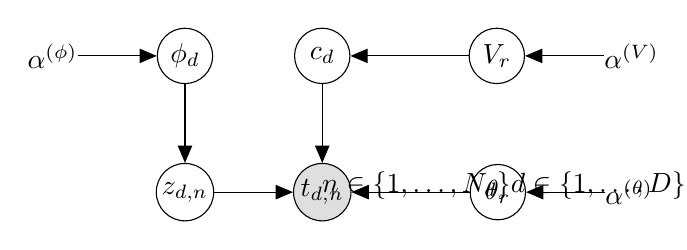
\begin{tikzpicture}
\node[obs] (t) {$t_{d,n}$};
\node[latent, above=of t] (c) {$c_d$};
\node[latent, right=1.5cm of c] (v) {$V_r$};
\node[latent, right=1.5cm of t] (th) {$\theta_r$};
\node[latent, left=of t] (z) {$z_{d,n}$};
\node[latent, above=of z] (phi) {$\phi_d$};
\node[const, left=of phi] (alphaPhi) {$\alpha^{(\phi)}$};
\node[const, right=of v] (alphaV) {$\alpha^{(V)}$};
\node[const, right=of th] (alphaTheta) {$\alpha^{(\theta)}$};

\edge{phi}{z};
\edge{z}{t};
\edge{c}{t};
\edge{v}{c};
\edge{th}{t};
\edge{alphaPhi}{phi};
\edge{alphaV}{v};
\edge{alphaTheta}{th};

\centeredPlate{word-plate}{(t)(z)}{$n \in \{1, \ldots, N_d\}$};
\centeredPlate{doc-plate}{(phi)(c)(z)(t)(word-plate)}{$d \in \{1, \ldots, D\}$};
\centeredPlate{tree-plate}{(th)(v)}{\begin{tabular}{c}$r: $ path to \\ any node\end{tabular}};
\end{tikzpicture}
%
\caption{Plate diagram for the NCRP topic model}
\label{fig:plate-ncrp}
\end{figure}
%%%%

We will see that, relative to the LDA model, the task of computing the posterior distribution in the NCRP model is complicated by the fact that there are infinitely many latent random variables (for example, there is one latent beta-distributed random variable for each node in the infinite tree).
The algorithms that have been proposed for inference in the NCRP topic model fall into two main categories: those based on Gibbs sampling, and those based on variational inference.

\subsubsection{Gibbs Sampling for the NCRP}

Initially, papers such as \cite{griffiths2004hierarchical}, used NCRP inference algorithms based on Gibbs sampling.
(In the next section, we will discuss an alternate inference algorithm that was introduced in \cite{wang2009vi_ncrp}.)
In Gibbs sampling, we maintain a state vector which stores values for each of the latent random variables.
Each iteration involves updating the state vector by sampling each of the latent variables, one at a time, according to the following conditional probabilities:
\begin{align}
z_k &\sim p(z_k \mid \vec x, \vec z_{-k}) \qquad \text{for all latent variables $z_k$.}
\end{align}
Here, $\vec z_{-k}$ represents the current state vector with the entry for $z_k$ omitted (that is, it represents the current state of all latent variables \emph{except} for $z_k$), and $\vec x$ represents all observed variables.
The long-term behavior of this stochastic system is guaranteed to approach the true posterior distribution, $p(\vec z \mid \vec x)$.
However, it can be difficult to determine whether the state vector has converged.
Moreover, the state vector only represents a single snapshot of the latent variables, as opposed to a distribution over the latent variables, and so we must collect a large number of state-vector samples.
The resulting collection of state-vector samples can then be used as an empirical approximation to the posterior distribution.
Issues such as burn-in (the number of samples to discard before saving the first sample) and lag (the number of samples to discard between saved samples, in order to avoid correlated samples) can also affect the performance of Gibbs sampling.

For some models, it is possible to omit some of the latent variables from the state vector.
This can be done by marginalizing the conditional probabilities over the omitted variables.
One common approach is to marginalize out any global variables (i.e., variables which are shared across all observed data points), leaving only ``local'' per-observation variables in the state vector.
This approach is known as ``collapsed Gibbs sampling,'' and it is used in \cite{blei2010ncrp}.

%**TODO-actual-algorithm??

\subsubsection{Variational Inference for the NCRP}

A variational inference algorithm for the NCRP model was proposed in \cite{wang2009vi_ncrp}.
In general, variational inference involves defining a restricted set of functions and searching for the member of that set which most closely approximates the function we wish to compute---in this case, the true posterior distribution.
This particular algorithm uses reversed Kullback-Leibler divergence to measure the distance between a candidate distribution and the true posterior.
In the paper by Wang et al, the set of approximating distributions $Q$ is the set of all functions which can be written in the following form:
\begin{align}
q(\vec z) = \prod_{k=1}^m q_k(z_k)
\end{align}
where $\vec z = (z_1, \ldots, z_m)$ represents the full set of latent variables in the model, and where each function $q_k$ is a member of a parameterized family of univariate distributions.
If we let $\nu_k$ represent the parameters associated with the $k\nth$ latent variable, then the function $q$ is fully specified by selecting a value for $(\nu_1, \ldots, \nu_m)$.
By assuming that the posterior can be approximated as a product of univariate factors, we use what is known as the ``mean-field approximation.''
In mathematical notation, if $p(\cdot \mid x)$ represents the true posterior distribution, we wish to find $q$ such that
\begin{align}
\mathcal L &= \text{KL}( q \;\Vert\; p(\cdot \mid x) )
\end{align}
is minimized.
By expanding the definition of $\mathcal L$, we can write
\begin{align}
\mathcal L &= \log p(x) - \text{ELBO},
\end{align}
where ELBO (short for ``evidence lower bound'') is defined as
\begin{align}
\text{ELBO} = E_q[\log p(\vec z, \vec x)] - E_q[\log q(\vec z)]
\end{align}
Then, since $\log p(x)$ does not depend on $q$, minimizing $\mathcal L$ is equivalent to maximizing ELBO.
This fact will be useful later when we wish to monitor the convergence of our algorithm, because ELBO is signficantly easier to compute than the actual objective function $\mathcal L$.

The actual update rules are derived using coordinate ascent; that is, we repeatedly update the latent variables, one at a time.
In particular, we derive the updates by computing the functional derivative of the objective function with respect to one of the latent variables and solving for the value of the corresponding variational parameter which makes this functional derivative equal to zero.
To aid in deriving the update rules, the model is typically constructed such that all distributions are members of the exponential family, and conjugate priors are used wherever possible.
This is, by design, true of the NCRP model.
Moreover, the variational distributions $q_k$ are assumed to belong to the same family as the corresponding model distribution $p(z_k \mid \text{parents}(z_k))$.

In general, the coordinate-ascent update rule can be derived by calculating the logarithm of the model's joint probability distribution and then performing the following steps for each latent variable $z_k$:
\begin{itemize}
\item Drop any constant terms in the log joint probability (that is, terms that do not depend on $z_k$).
\item Express the remaining terms as a dot product between the ``sufficient statistics'' of the distributon $p(z_k \mid \text{parents}(z_k))$, which are functions of $z_k$, and a vector of ``natural parameters,'' denoted $\eta_k$, which do not depend on $z_k$.
\item Compute the expectation of $\eta_k$ with respect to the variational distributions for the latent variables.
That is, compute
\begin{align}
E_q[\eta_k] &= E_{z_1 \sim q_1} \left[ \cdots E_{z_m \sim q_m} \left[ \eta_k \right] \cdots \right]
\end{align}
\item Compute the inverse of the natural parameter transformation corresponding to the variational distribution $q_k$, and apply it to the vector $E_q[\eta_k]$.
This yields the concrete values with which to update the variational parameters corresponding to $z_k$.
\end{itemize}
We then repeat the above steps while continually monitoring the value of the ELBO until it appears to have converged.

The above procedure is sufficient for traditional finite-dimensional models.
However, in the context of Bayesian nonparametric models such as the NCRP, the latent variables belong to an infinite-dimensional space.
This means that there are an infinite number of variational parameters that would need to be updated in each iteration.
Hence, in order to obtain a feasible algorithm, we must make additional approximations.
The approach taken in \cite{wang2009vi_ncrp} is to start with a finite version of the tree which has been truncated in terms of both its depth and its width.
The latent variables associated with the nodes that lie outside of this finite truncation are assumed to be equal to the corresponding prior distribution; thus, outside of the finite truncation, there is no dependence on the variational parameters.
In addition to this, the authors also incorporate greedy heuristics for pruning paths, adding paths, and merging paths in the finite tree.

%***TODO-update-rules-specific-to-NCRP??

Compared to Gibbs sampling, variational inference has the advantange of being deterministic, and its convergence is also significantly easier to detect.
However, variational inference does have its own disadvantages.
Whereas with Gibbs sampling, it is possible to approach the true posterior distribution to an arbitrary level of precision, variational inference can only yield an approximation.
When deriving variational updates, we face a tradeoff: we can choose a more restricted set of variational distributions, which yields an inferior approximation, but leads to easier-to-derive update rules.
On the other hand, if we want a tighter approximation, the update rules are likely to be significantly more complicated.

\subsection{The Nested Hierarchical Dirichlet Process}

The primary limitation of the NCRP has to do with the fact that each document is associated with only a single path through the topic hierarchy.
This creates problems when the training corpus contains documents with a variety of ``hybrid'' topics.
From the example mentioned earlier, there may be some documents which are a mixture of \emph{sports} and \emph{medicine}, and the relative proportions of these topics may vary depending on the specific focus of the document.
To accommodate such documents, the NCRP leaves us with limited options:
\begin{enumerate}
\item Treat \emph{sports medicine} as a subtopic of either \emph{sports} or \emph{medicine}.
\item Treat \emph{sports medicine} as a top-level topic, distinct from both \emph{sports} and \emph{medicine}.
\end{enumerate}
Option 1 may lead to unmanageably deep topic hierarchies (or, if we are using the finite-depth variant of NCRP, this option may not even be feasible).
On the other hand, option 2 may lead to unmanageably wide topic hierarchies, particularly if a large number of documents are hybrids of three or more topics.
In either case, it becomes difficult to represent the topic hierarchy as a relatively small tree.

Rather than face these limited options, we would prefer to augment the model so that it can better handle a variety of hybrid topics.
The solution that was proposed in \cite{paisley2015nhdp} is a topic model called the Nested Hierarchical Dirichlet Process (NHDP).
The NHDP topic model shares many features in common with the NCRP topic model:
\begin{itemize}
\item Once again, we draw a global distribution over paths from an NCRP distribution.
\item As before, there is an infinite set of topic vectors (i.e., distributions over vocabulary words) which are arranged in an infinite tree and are independently drawn from a Dirichlet distribution.
\item Furthermore, each document is associated with a ``local'' distribution over nodes in the infinite tree of topics.
\end{itemize}
The main difference between these two topic models is the way in which the local distribution over nodes is defined.
In the NCRP topic model, each document's local distribution consists of nodes along a single path, but in the NHDP, the local distributions can include multiple branches.
This is designed to address the previously-mentioned limitation regarding documents that exhibit a wide variety of hybrid topics.

To see how the local, per-document distributions are defined in the NHDP, we must first discuss the (non-nested) Hierarchical Dirichlet Process (HDP).
The HDP was introduced in \cite{teh2005hdp} to model grouped data, in which there are an unbounded (potentially infinite) number of groups, each of which contains multiple observations and is associated with its own vector of parameters.
A simple, non-nested HDP model can be formulated as follows:
\begin{align}
H &\sim \text{DP}(\alpha, G_0) \\
H_d &\sim \text{DP}(\beta, H) \\
\mu_{d,n} &\sim H_d \\
x_{d,n} &\sim F(\mu_{d,n})
\end{align}
In this formulation, there is a base distribution $G_0$ (such as a Gaussian or a Dirichlet), and a ``global'' distribution $H$ is drawn from a Dirichlet process applied to $G_0$.
The distribution $H$ is discrete, which means that can be viewed as a distribution over countably many independent draws from the base distribution.
Next, per-group distributions $H_d$ (one for each group $d$ in the data) are drawn from another Dirichlet process, which is applied to the global distribution $H$.
For each data point $n$ in group $d$, a parameter vector $\mu_{d,n}$ is drawn from the group-specific distribution $H_d$.
Finally, the observed data points $x_{d,n}$ are drawn according to the distribution $F(\mu_{d,n})$, where $F$ is some parameterized distribution, such as a Gaussian or a categorical distribution.
In the context of topic models, a ``group'' is often defined to be a single document, and the individual observations within each group are the words within the corresponding document.
The NHDP model uses $G_0 = \text{Dirichlet}(\gamma)$ and $F(\cdot) = \text{Categorical}(\cdot)$.

To define a per-document distribution over nodes, the NHDP uses an HDP defined at each node of the infinite topic tree.
However, it also interleaves a document-specific tree of ``path propagation'' random variables to determine, for each word, whether to extend the current path by drawing the next subtopic or to stop at the current node and draw a specific vocabulary word.

The generative process is as follows:
\begin{outline}[enumerate]
\1 For each node $r$ in the infinite tree, draw a topic vector $\theta_r$, representing a distribution over the vocabulary.
Since this involves an infinite number of random draws, this step is performed via lazy evaluation.
\1 For each node $r$ and each $j \geq 1$, draw a beta-distributed stick-breaking proportion $V^*_{r,j}$ via lazy evaluation:
\1 For each document $d$:
  \2 For each node $r$ in the infinite tree, perform the following steps via lazy evaluation:
    \3 For each $j \geq 1$:
      \4 Draw an index $z^d_{r,j} \geq 1$ according to a discrete distribution with probabilities given by $\pi_k = V^*_{r,k} \prod_{i=1}^{k-1} (1-V^*_{r,i})$.
      \4 Draw a beta-distributed stick-breaking proportion $V^d_{r,j}$.
    \3 Draw a beta-distributed path-propagation random variable $U^d_r$.
  \2 For each word-slot $n$ in document $d$:
    \3 Let $r = ()$, the empty path.
    \3 Repeat the following steps until a value for $c^d_n$ is chosen:
      \4 Draw a Bernoulli random variable with probability of success $U^d_r$.
      \4 If the outcome is 1, then set $c^d_n = r$ and break out of this loop; otherwise, continue.
      \4 For all $j \geq 1$ (via lazy evaluation), find all indices $k$ such that $z^d_{r,k} = j$.  Let $S_j$ be the set of such indices, and define $\mu_j = \sum_{k \in S_j} V^d_{r,k} \prod_{i=1}^{k-1} (1-V^d_{r,i})$.
      \4 Draw an index $\tilde z \geq 1$ from a discrete probability distribution with probabilities given by $\mu_j$ as defined above.
      \4 Extend $r$ by appending $\tilde z$ to it; that is, update $r \gets (r, \tilde z)$.
    \3 Draw a vocabulary word $t^d_n$ from a categorical distribution with probabilities given by $\theta_{c^d_n}$.
\end{outline}

In summary, we first draw an infinite, global tree of topics ($\theta_r$) and stick-breaking proportions ($V^*_{r,j}$).
Then, for each document $d$, we draw local sequences of indices ($z^d_{r,j}$) based on the global stick-breaking proportions.
We also draw an independent set of document-specific stick-breaking proportions ($V^d_{r,j}$).
Together, $z^d_{r,j}$ and $V^d_{r,j}$ determine how the topics descended from node $r$ are rearranged and re-weighted in a document-specific fashion.
Furthermore, we draw ``path-propagation'' probabilities $U^d_r$ for each document, and for each node in the infinite tree.
By combining $z^d_{r,j}$, $V^d_{r,j}$, and $U^d_r$, we have a per-document distribution over an infinite tree of nodes.
For each word $n$ in a given document $d$, we draw a node $c^d_n$ from this document-specific distribution over nodes;
this identifies the topic from which the $n\nth$ word of document $d$ will be drawn.
Finally, we draw a vocabulary word $t^d_n$ from ${\text{Categorical}(\theta_{c^d_n})}$.

To visualize how the NHDP model is constructed, Figure~\ref{fig:plate-nhdp} contains a plate diagram of the Bayesian network underlying this model.
Figure~\ref{fig:prob-nhdp} shows the corresponding conditional probability distributions.

%%%%
\begin{figure}[htb]
%
\centering
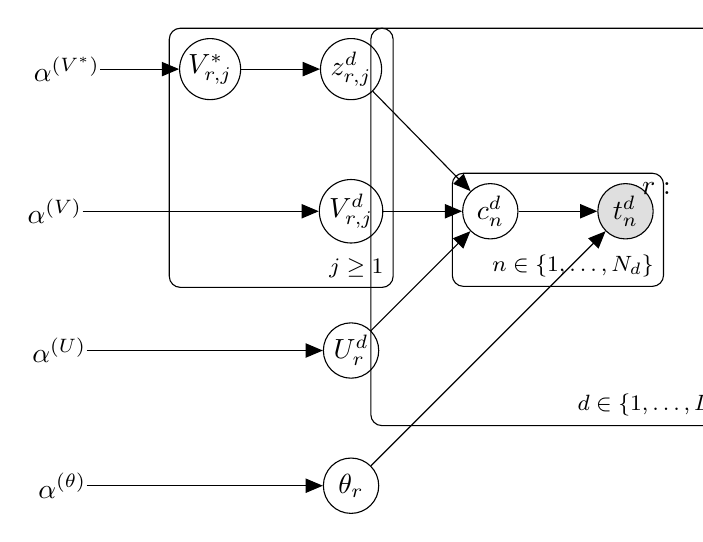
\begin{tikzpicture}
\node[obs] (t) {$t^d_n$};
\node[latent, left=of t] (c) {$c^d_n$};
\node[latent, left=of c] (v) {$V^d_{r,j}$};
\node[latent, below=of v] (u) {$U^d_r$};
\node[latent, above=of v] (z) {$z^d_{r,j}$};
\node[latent, left=of z] (vstar) {$V^*_{r,j}$};
\node[latent, below=of u] (th) {$\theta_r$};
\node[const, left=of vstar] (alphaVstar) {$\alpha^{(V^*)}$};
\node[const, left=3cm of th] (alphaW) {$\alpha^{(\theta)}$};
\node[const, left=3cm of v] (alphaV) {$\alpha^{(V)}$};
\node[const, left=3cm of u] (alphaU) {$\alpha^{(U)}$};
%
\edge{c}{t};
\edge{z}{c}
\edge{v}{c};
\edge{u}{c};
\edge{vstar}{z};
\edge{th}{t};
\edge{alphaV}{v};
\edge{alphaU}{u};
\edge{alphaVstar}{vstar};
\edge{alphaW}{th};
%
\plate{word-plate}{(t)(c)}{$n \in \{1, \ldots, N_d\}$};
\plate{j-plate}{(z)(vstar)(v)}{$j \geq 1$};
\centeredPlate{tree-plate}{(u)(v)(z)(th)(vstar)(j-plate)}{\begin{tabular}{c}$r: $ path to \\ any node\end{tabular}};
\plate{doc-plate}{(word-plate)(z)(u)(v)}{$d \in \{1, \ldots, D\}$};
\end{tikzpicture}
%
\caption{Plate diagram for the NHDP topic model}
\label{fig:plate-nhdp}
\end{figure}

\begin{figure}[htb]
\centering
\begin{empheq}[box=\fbox]{align*}
\theta_r &\sim \text{Dirichlet}(\alpha^{(\theta)}) \\
V^*_{r,j} &\sim \text{Beta}(1, \alpha^{(V^*)}) \\
V^d_{r,j} &\sim \text{Beta}(1, \alpha^{(V)}) \\
U^d_r &\sim \text{Beta}(\alpha^{(U)}_1, \alpha^{(U)}_2) \\
z^d_{r,j} &\sim \sum_{k \geq 1} \left( V^*_{r,k} \prod_{i=1}^{k-1} (1-V^*_{r,i}) \right) \delta_k \\
c^d_n &\sim \sum_{r: \text{path}} A(r, V^d, z^d) \, B(r, U^d) \, \delta_r \\
A(r, V^d, z^d) &= \prod_{m=0}^{\len(r)-1} \sum_{k \geq 1} \indicator \left[ z^d_{r[1:m],k} = r[m+1] \right] \left( V^d_{r[1:m],k} \prod_{i=1}^{k-1} \left( 1 - V^d_{r[1:m],i} \right) \right) \\
B(r, U^d) &= U^d_r \prod_{m=0}^{\len(r)-1} \left( 1 - U^d_{r[1:m]} \right) \\
t^d_n &\sim \text{Categorical}(\theta_{c^d_n})
\end{empheq}
\caption{Conditional probability distributions for the NHDP topic model}
\label{fig:prob-nhdp}
\end{figure}

\subsubsection{Variational Inference for the NHDP}

The inference algorithm for the NHDP model is again based on variational inference.
However, the authors use a variant called \emph{stochastic variational inference} (which was introduced in \cite{hoffman2013stochastic}) to allow the algorithm to scale to larger datasets.
This approach uses repeated sampling of mini-batches to update the variational parameters, and in this respect it is similar to stochastic gradient descent.
The update rules for document-specific variables are the same as in traditional variational inference, but the ``global'' (i.e., corpus-wide) variables are updated using the \emph{natural gradient} of the objective function.

Using a standard gradient makes sense in cases where we can judge whether two candidate maximizers are sufficiently close to each other based purely on Euclidean distance.
However, in the case of parameterized probability distributions, the Euclidean distance between pairs of parameter vectors may not accurately reflect the ``true'' difference between the corresponding probability distributions.
Hoffman \cite{hoffman2013stochastic} gives an example involving a normal distribution parameterized by its mean and variance.
If we start with a mean of $\mu = 0$ and a variance of $\sigma^2 = 0.01$, then adding $1$ to the mean will have a relatively large effect, since $\mathrm{Normal}(0, 0.01)$ has very little overlap with $\mathrm{Normal}(1, 0.01)$.
The situation is reversed if we start with $\mu = 0$ and $\sigma^2 = 1000$, since $\mathrm{Normal}(0, 1000)$ is nearly identical to $\mathrm{Normal}(1, 1000)$.
Thus, relying on gradients defined in terms of Euclidean distance can lead to unnecessarily slow convergence, since some steps will essentially be wasted by moving in an inefficient direction.

To address this, we define a matrix $G$ which encodes information about how the ``true'' distance function varies within a local neighborhood.
This matrix $G$ is also known as a \emph{metric tensor}.
When dealing with parameterized probability distributions, we can define $G$ in terms of a symmetric variant of KL divergence.
Then, rather than simply following the gradient of the objective function in Euclidean coordinates (i.e., $\nabla \mathcal L$), the natural gradient takes steps in direction of $G^{-1} \nabla \mathcal L$.
The natural gradient update rule has a particularly simple form for exponential-family models, since the metric tensor corresponding to symmetrized KL divergence conveniently cancels with part of gradient of the objective function in such cases.
We are then left with a formula that agrees with the coordinate-ascent update rules.

Furthermore, instead of computing the gradient of the objective function based on the entire dataset, we can use stochastic optimization techniques to compute updates based on mini-batch sampling.
As long as we base our updates on estimates which agree with the natural gradient \emph{in expectation}, we will still achieve reasonable convergence.
(The same principle is at work in stochastic gradient descent.)
Stochastic variational inference accomplishes this by repeatedly sampling mini-batches of documents.
For each document in each mini-batch, the local per-document parameters are updated according to the traditional coordinate-ascent formulas.
For the global parameters, only a small change is needed: we compute the variational-parameter updates as if the mini-batch had been scaled up to the size of the full dataset.
In other words, if the full dataset has $D$ documents, and a mini-batch contains $S$ documents, with $S \ll D$, we perform updates for the global parameters using a virtual dataset consisting of $D / S$ copies of the mini-batch.

By using stochastic variational inference, we end up with an algorithm which is, in practice, more efficient than either Gibbs sampling or coordinate-ascent variational inference.
This is because this algorithm typically requires fewer iterations through the full dataset.
In particular, it allows us to update our estimates for the global (corpus-wide) latent variables more frequently than once per iteration through the dataset.
%**TODO-vi-algorithm-for-nhdp?

%%%%%%%%%%%%%%%%%%%%%%%%%%%%%%%%
\section{Directions for Future Research}

We can identify some directions for future research by considering some of the limitations of the NHDP topic model.

\paragraph{Scalable algorithms:}
The currently available set of inference algorithms force us to make a significant tradeoff between precision and scalability.
On the one hand, we have Gibbs sampling, which can theoretically compute the true posterior distribution with arbitrary precision, but which requires requires many passes over the training data and therefore fails to scale well to massive datasets.
On the other hand, we have stochastic variational inference, which uses a more efficient mini-batch approach and has deterministic convergence; however, it requires us to make major approximating assumptions, such as the mean-field approximation.
To improve the inference algorithm, we could perhaps look for a variant of Gibbs sampling that requires fewer passes over the training data.
Alternatively, we might seek a modified version of stochastic variational inference which makes less stringent assumptions on the form of the variational distributions.
Yet another approach might be to extend the non-probabilistic, geometric ``anchor words'' approach of Arora et al \cite{arora2013practical} in order to handle hierarchies of topics.

\paragraph{Interpreting models:}
The models discussed above generally represent topics as discrete probability distributions over the entire vocabulary.
However, a typical vocabulary may contain tens of thousands of words, which makes the vector of topic probabilities unwieldy and difficult to interpret.
A common approach is to visualize a topic by displaying its top $K$ most likely vocabulary words.
However, within a large topic hierarchy, a small value of $K$ might not provide enough information to disambiguate closely related topics, whereas a large value may lead to information overload.
By comparison, human-curated topic hierarchies such as library cataloguing systems often use a very small number of words to describe each node in a large hierarchy.
Hence, it might be useful to develop techniques to post-process the results of these models in order to derive a concise yet meaningful description of each topic.

\paragraph{Incorporating human feedback:}
In cases where the model's quality is deemed subpar, it may be useful to be able to incorporate human feedback.
This would require not only an investigation of the types of mistakes which these topic models are prone to make in practice, but also an investigation into how best to design a user interface that is capable of gathering useful feedback.
It may also be useful to apply semi-supervised or multi-label classification techniques in scenarios where partial or even contradictory labels are available.

\paragraph{Moving beyond the bag-of-words model:}
All of the models discussed above ignore the order in which words appear in a document.
The sequence of words in a document can influence its meaning, and therefore its classification within a topic hierarchy.
By making use of word-order information, we could potentially improve the quality of the results.

\paragraph{Frameworks for Bayesian non-parametric inference:}
Deriving inference algorithms for Bayesian non-parametric models, such as the ones discussed above, is a laborious process which is difficult to automate.
For instance, even though the NCRP and NHDP topic models share many features, their inference algorithms must be derived in a model-specific way.
This is made especially difficult by the fact that, in Bayesian non-parametric models, there can be an infinite number of latent variables.
This requires us to augment traditional inference algorithms with model-specific heuristics.
An approach that combines black-box inference techniques (such as those described in \cite{ranganath2014blackbox} and \cite{ranganath2016operator}) with model-agnostic heuristics for handling infinite-dimensional latent variables might make it feasible to efficiently explore and compare many variants of these models.

%%%%%%%%%%%%%%%%%%%%%%%%%%%%%%%%
\clearpage
\nocite{*}
%\bibliographystyle{plainnat}
\bibliographystyle{plain}
\bibliography{../bibliography}

\end{document}
